\chapter{Mesoscale signatures of the North Atlantic Oscillation and interaction with the ocean}

% **************************** Define Graphics Path **************************
%\ifpdf
%    \graphicspath{{Chapter3/Figs/Raster/}{Chapter3/Figs/PDF/}{Chapter3/Figs/}}
%\else
%    \graphicspath{{Chapter3/Figs/Vector/}{Chapter3/Figs/}}
%\fi
% Each path has to end with a / and be enclosed in curly braces { } even if only one path is specified. 
\graphicspath{{Chapter4/Figs/}}


%: shear instability and air-sea interactions

Additions in thesis from paper:
Large-scale EKE
ERA-Interim results
More PV results, e.g. histograms, isentropic in ERA5 and ERAI, pressure levels in ERA5
Heat flux
Sheldon paper as motivation rather than results
PV in results rather than discussion
Negative shear, buoy, etc?



%%%%%%%%%%%%%%%%%%%%%%%%%%%%%%%%%%%%%%%%%%%%%%%%%%%%%%%%%%%%%%%%%%%%%%%%%%%%%%
\section{Introduction}

In the North Atlantic, the leading mode of winter climate variability is the North Atlantic Oscillation (NAO), which is related to sea surface temperature (SST) and storm track activity \citep{vallis2008local}. The large-scale tripole of SST associated with the positive NAO phase (NAO+) has been discussed in many observational and modeling studies (e.g. \citet{bjerknes1964atlantic}, \citet{wallace1987observed}, \citet{czaja2001observations}, \citet{peng2002north}, \citet{visbeck2003ocean}). In both obs and models this is at a coarse resolution (>200km). Summary from these studies is Kushnir et al. 2002: suggestion of weak positive feedback of tripole onto NAO but predominantly one way forcing of the ocean by the atmosphere. The Gulf Stream is related to NAO phase by affecting the eddy driven jet and associated extra-tropical cyclones \citep{sampe2010significance, nakamura2008importance, booth2012sensitivity, small2014storm, woollings2012response, vanniere2017contribution, vanniere2017cold}. Further to such work on large-scale signals, the focus of this study is to examine whether there also exists a mesoscale signature. This is being investigated by analyzing variables smaller than 100 km, reflecting processes that are occurring within the synoptic scale extra-tropical cyclones. With the production of new, higher resolution datasets, we can investigate whether there are also NAO signals in the atmosphere and ocean on smaller scales. 

Many studies have examined air-sea interactions associated with western boundary currents  \citep{ma2015distant, shaman2010air, kwon2010role, czaja2001observations, czaja2002observed, minobe2008influence, smirnov2015investigating, kelly2010western, cayan1992latent}, and it has been shown that the Gulf Stream plays an important role in the climate of the northern hemisphere, mainly through affecting the eddy driven jet and associated extra-tropical cyclones \citep{sampe2010significance, nakamura2008importance, booth2012sensitivity, small2014storm, woollings2012response, vanniere2017contribution, vanniere2017cold}. Further to such work on large-scale signals, the focus of this study is to examine whether there also exists a mesoscale signature. This is being investigated by analyzing variables smaller than 100 km, reflecting processes that are occurring within the synoptic scale extra-tropical cyclones.

Visbeck chapter: "However, outside of the deep tropics, most studies find that the ocean largely reacts to the high frequency changes of the atmospheric forcing and that its influence back to the atmosphere is weak on time scales shorter than a decade."

%%%%%%%%%%%%%%%%% Sheldon %%%%%%%%%%%%%%%%%%%%%%%%

Woollings 2010 winter.
%In a modeling study using a 12 km grid, \citet{sheldon2017warm} showed that the Gulf Stream warm tongue affects atmospheric shear production.  

In a modeling study of an extratropical cyclone, \citet{sheldon2017warm} showed that the Gulf Stream warm tongue affects atmospheric instability? energy production?.  When a strong Gulf Stream warm tongue was present, shear production was found downstream, but in an experiment where the SST is smoothed, the shear production is reduced (figures \ref{fig:Sheldon}). Along with this signal in shear production, they found a region of negative PV at mid-levels associated with the warm tongue, and lack of this in a smooth set up.This experimental study of a single storm suggests that the Gulf Stream warm tongue anchors shear production.

\begin{figure}[h]
	\centering
	\includegraphics[width=14pc]{Arnaud_plot.PNG}
	\caption{Distribution of shear production (in mW/kg) at height z=4.5 km 24 hours into the model run. (a) control (b) smooth. The associated SST distributions are shown in black contours. Further work from analysis \citet{sheldon2017warm}.}
	\label{fig:Sheldon} 
\end{figure}


In this study, we use high resolution reanalyses to examine buoyancy and shear production, as well as SST and surface currents during boreal winter and establish whether there exists a relationship with NAO phase.

\todo{Sort references here. Added Cayan but not yet read this paper. Visbeck et al 2000  2003?}

%Suggestions that synoptic scale could feed back onto large-scale. What about mesoscale 
%(To analyse the mesoscale signature in both the ocean and atmosphere, to assess air-sea interactions and they relationship with the NAO.
%Furthermore, by comparing two reanalysis datasets, allows assessment into the role of model resolution on this process.)
%We show that there is a signal and propose that this is related to the Gulf Stream warm tongue.

%It has been suggested (Woollings, etc) that the NAO is related to negative PV, and this study is motivated by Sheldon to examine if this shear diagnostic has a signal in the NAO.

%Further investigation into the effect of the SST on shear instability in these reanalysis products.
%Observational study using reanalyses

%intensity or amount or strength

%\citet{minobe2008influence} found that it affects the entire troposphere. 
%\citep{czaja2011new} - oceans influence the atmopshere through convection in midlatitudes, which is commonly occurring in Tropics.
%ocean on atmosphere in mid-lats, rather than atm on ocean. 


%The atmosphere may be inertially stable to horizontal displacements and gravitationally unstable to vertical displacements, but may be unstable to slantwise displacements by shear instability. It has been suggested that slantwise convection from the release of (moist symmetric)shear instability can explain banded precipitation often seen at cold fronts \citep{bennetts1979conditional, seltzer1985possible, emanuel1983lagrangian, emanuel1983assessing, morcrette2006formation, chen2018assessment}, caused by cells of alternating rotation creating updrafts and downdrafts.

%Much analysis with ERA-Interim, but new ERA5 is higher resolution with other model improvements.

%Atmospheric reanalyses are a valuable tool for weather and climate analysis and are often treated as the best-guess truth. New improved reanalyes are released generally at increased resolution with other improvements such as to the data assimilation scheme and parametrisations.

%warm conveyor belts

%Shear (or symmetric) instability is a combination of gravitational and inertial instability. A parcel may be inertially stable to horizontal displacements and gravitationally stable to vertical displacements, but may be unstable to slantwise displacements by shear instability. The  M-$\theta$e relationship states that if the $\theta$e surfaces are steeper than the M surfaces, there is symmetric instability. Any slantwise displacement occurring between the slopes of these surfaces will release the symmetric instability and the parcel will be accelerate in the direction away from the original position. Only moist slantwise instability occurs in the Earth's atmosphere \citep{bennetts1979conditional} and so $\theta$e is used. This instability has a 2D assumption that there is no variation in the along front direction.

% 2D theory \citet{eliassen1962vertical}
%%%%%%%%%%%%%%%%%%%%%%%%%%%%%%%%%%%%%%%%%%%%%%%%%%%%%%%%%%%%%%%%%%%%%%%%%%%%%%%%
\subsection{ Hypothesis / Aim}



\section{Data and Methodology}

We use two reanalysis datasets produced by ECMWF (European Centre for Medium-Range Weather Forecasts). ERA-Interim spans 1979-present and has a spatial resolution of 0.75$^{0}$ \citep{dee2011era}. The new ERA5 reanalysis is the 5th major global reanalysis produced by ECMWF and has a finer resolution of 0.25$^{0}$ alongside other model improvements, including increased temporal resolution (ref). The period analyzed is December, January and February, for 5 positive NAO and 2 negative NAO years. The selection of positive and negative NAO years was made using NAO Index Data provided by the Climate Analysis Section, NCAR, Boulder, USA, Hurrell (2003). From 2008 to 2017, when both the station and principal component time series data of sea level pressure agree on sign of NAO index, this year was selected. The 5 positive NAO years (2011-12, 2013-14, 2014-15, 2015-16, 2016-17) and 2 negative NAO years (2009-10, 2010-11) are independent.
%Updated regularly. Accessed DD Month YYYY [list date you accessed the data].

  \begin{table}
  \caption{NAO positive and negative winters} \label{t_NAO}
  \centering
  \begin{tabular}{c c c c c c}
  \hline
  \textbf{Positive} & 2011--2012 & 2013--2014 & 2014--2015 & 2015--2016 & 2016--2017 \\
  \hline
  \textbf{Negative}  & 2009--2010  & 2010--2011 &  &  &  \\
  \hline
  \end{tabular}
  \end{table}


%Across each winter, there are 2184 (+x for leap year) time steps. (mean this)

 \begin{figure}[h]
 	\centering
 	\includegraphics[width=26pc]{NAO_TS_scatter_norm.pdf}
 	\caption{NAO}
 	\label{fig:NAO_TS}
 \end{figure}

The diagnostics are production terms for mesoscale kinetic energy. A spatial filter over a region of 3 degrees (\textasciitilde{300} km) was applied to the data to obtain the high-pass prime values and low-pass bar values, covering 13 and 5 grid points for ERA5 and ERA-Interim, respectively. This is to separate the low frequency background from the high frequency perturbations and to examine small scale has an effect on the large scale. 

\begin{equation} \label{eq_diag1}
\frac{\partial}{\partial{t}} \Bigg(\frac{\overline{u'^2 + v'^2}}{2}\Bigg) = \text{Shear production + Buoyancy production} + ... 
\end{equation}

\begin{equation} \label{eq_diag2}
\text{Shear production} \,(mWkg^{-1}) = -\Bigg({\overline{w'u'} . \frac{\partial{\overline u}}{\partial z} + \overline{w'v'} . \frac{\partial{\overline v}}{\partial z}}\Bigg)
\end{equation}

\begin{equation} \label{eq_diag3}
\text{Buoyancy production} \,(mWkg^{-1}) = {-\overline{w'\alpha'}}
\end{equation}

Don’t forget the BP term in your MKE equation is for pressure coordinate.

Buoyancy is calculated using specific volume ($\alpha$), defined using density from temperature, and u, v, and w, represent zonal, meridional and vertical velocities. Remaining terms denoted by ellipsis include friction. (Averages over DJF are averaged again to give NAO+ and NAO-.)

The instability in the x (u) and y (v) directions are combined. The covariance of small-scale vertical motions ($\omega$') and horizontal vertical motions (u' or v') is calculated and then the  product with the vertical shear of low pass winds ($\overline{u}$ or $\overline{v}$)  is created. The high pass, to capture the high variability, was original minus low pass. 
computed over the North Atlantic domain (20-80N, 90W-40E).

Twelve pressure levels were used for this analysis (200, 300, 400, 500, 600, 700, 800, 850, 875, 900, 925, 950 hPa), with the lowest and highest omitted from the shear diagnostic calculation as they require another level from which to calculate the shear term. Values are then interpolated (linearly) to every 25 hPa, giving 31 levels in total, and 26 for shear production. In this analysis, integration across levels 300-600 hPa and 625-925 hPa are classified as upper and lower levels, respectively. When integrated across levels (multiplied by dp/g * 1000) both production terms have the units Wm$^{-2}$. 

The SSTs used in both ERA5 and ERA-Interim for the period (2008-present) are from the Operational Sea Surface Temperature and Sea Ice Analysis (OSTIA), which has a resolution of 0.05$^{0}$ \citep{donlon2012operational}. OSCAR (Ocean Surface Current Analysis Real-time) \citep{Bonjean2002} contains near-surface ocean current estimates, on a 0.33$^{0}$ grid. Horizontal velocity is estimated from sea surface height, surface vector wind and SST from satellites and in situ instruments in a model combining geostrophic, Ekman and Stommel shear dynamics, and a complementary term from the surface buoyancy gradient. The temporal resolution of variables used from ERA5, ERA-Interim and OSCAR are 1-hourly, 6-hourly and 5-day, respectively.

%However, all these studies were limited to one ora few single events rather than a climatology and the systematicpresence of negative PV in the cold sector has, to our knowledge,never been explored. Negative PV in the cold sector of baroclinicstorms may have received little attention, because it is not includedin classical models of cyclogenesis (e.g. the Eady model has PVequal to 0 uniformly) and because anomalous PV is more oftendiagnosed than PV itself.

%https://podaac.jpl.nasa.gov/dataset/OSCAR_L4_OC_third-deg

%(The variables are instantaneous, defined as from the last model time step (ref ECMWF), which is 30 minutes in ERA-Interim and 15 minutes in ERA5.)

% ERA5 uses the same 37 pressure levels as ERA-Interim.

%Just compare ERA-Interim with ERA-5. For a fair comparison, use ERA5 at same time resolution as ERA-Interim

%%%%%%%%%%%%%%%%%%%%%%%%%%%%%%%%%%%%%%%%%%%%%%%%%%%%%%%%%%%%%%%%%%%%%%%%%%%%%

\section{Results}

In the ERA5 reanalysis, embedded in the large-scale SST tripole is a mesoscale structure to the east of Cape Hatteras, with a warming of ~3$^{0}$C in NAO+ (figure \ref{fig:subplot1}). Examination of surface currents from OSCAR \citep{Bonjean2002} shows that there is an acceleration along the axis of the warm tongue in the NAO+ compared to NAO- and a northward shift (figure \ref{fig:subplot1}). The mean surface current speed over 8 boreal winters (5 NAO+, 2 NAO-, 1 neutral) (contour line in figure \ref{fig:subplot1}), is 0.5ms$^-$$^1$ which is comparable to the magnitude of the anomalies. This suggests a very significant change of the current. Geostrophic / Ekman? energy. Forced by the geostrophic current = OSCAR rather than surface fluxes or Ekman fluxes. Relationship between current speed and warming / shift. Examination of the oceanic column (figure \ref{fig:ARGO}) (IN NAO+?) shows a shallow signature of warmer (and fresher) water reflecting the SST tripole, and also reveals a warm and saline (salty?) anomaly extending deeper around 37N, which seems to represent a poleward shift of the mean temperature/salinity front, reinforcing the coupled nature of the problem and the importance of ocean dynamics, current and SST.

\begin{figure}[h]
	\centering
	\includegraphics[width=24pc]{sst_current_subplot.pdf}
	\caption{a) Difference in SST between positive NAO and negative NAO years. b) SST distribution  in positive and d) negative NAO years. d) Difference in surface currents NAO positive - NAO negative. Contour line mean 0.5m/s? current over all winters (2009-10 to 2016-17). SST data from hourly ERA5 reanalysis. Surface current data from OSCAR, 5-day temporal resolution. Seasonal mean (DJF)}
	\label{fig:subplot1} 
\end{figure}

\begin{figure}[h]
	\centering
	\includegraphics[width=22pc]{ARGO_temp.png}
	\caption{ARGO}
	\label{fig:ARGO. CITE ARNAUD} 
\end{figure}


%%%%%%%%%%%%%%%%%%%%%%%%%%%%%%%%%%%%%%%%%%%%%%%%%%%%%%%%

Following results shown are positive production terms (equations \ref{eq_diag2}, \ref{eq_diag3}) calculated from hourly ERA5 reanalysis data over the winter season (DJF), averaged over the years in each NAO phase. The warm tongue is narrower and warmer in NAO+, with the 21 $^{0}$C isotherm approximately collocated with the 20 $^{0}$C isotherm (figure \ref{fig:subplot1}). The 21 $^{0}$C isotherm is shown in figures \ref{fig:ERA5_buoy} and \ref{fig:ERA5_shear}.

We recover the standard north-south dipole in classic variables such as U at 300hPa or EKE 

\begin{figure}[h]
	\centering
	\includegraphics[width=20pc]{ERA5_EKE200_subplot.pdf}
	\caption{Large scale time mean EKE at 200 hPa for a) positive and b) negative NAO years from hourly ERA5 data. NEED TO FILTER < 10day}
	\label{fig:ERA5_EKE200_NAO}
\end{figure}


In NAO+, the magnitude of buoyancy is approximately 20\% higher in the lower atmosphere (600-925 hPa) than the upper atmosphere (300-600 hPa), whereas in NAO- the magnitude is more consistent (figure \ref{fig:ERA5_buoy}). The spatial distribution shows differences with NAO phase, with an increase at higher latitudes and decrease in lower latitudes in NAO+, related to the expected shift of synoptic activity. At low levels over the Gulf Stream, there is a southwest-northeast dipole embedded in the large scale north-south shift. In NAO+, there is a displacement of buoyancy northeastwards along the warm tongue, suggesting an anchoring of this production term by the warm tongue. 

COME BACK TO THIS AFTER LOOKING AT HEAT FLUX AND LARGE-SCALE BUOYANCY:
This reflects the more extensive presence of warm water, opposing the expectation from more cold air outbreaks in NAO- (shown in numerous studies, eg .... \citep{fletcher2016climatology}). NO - SEE HEAT FLUXES, the opposite.
Stronger surface heat flux in NAO- (supplementary), especially over GS warm tongue area, more cold air outbreaks. SLHF twice as strong as SSHF. aligned with GS warm tongue

%The heat loss in the Labrador Sea in the positive NAO years is consistent. 
%The lower atmosphere more intense than the upper atmosphere, 
'diabatic'

\begin{figure}[h]
	\centering
	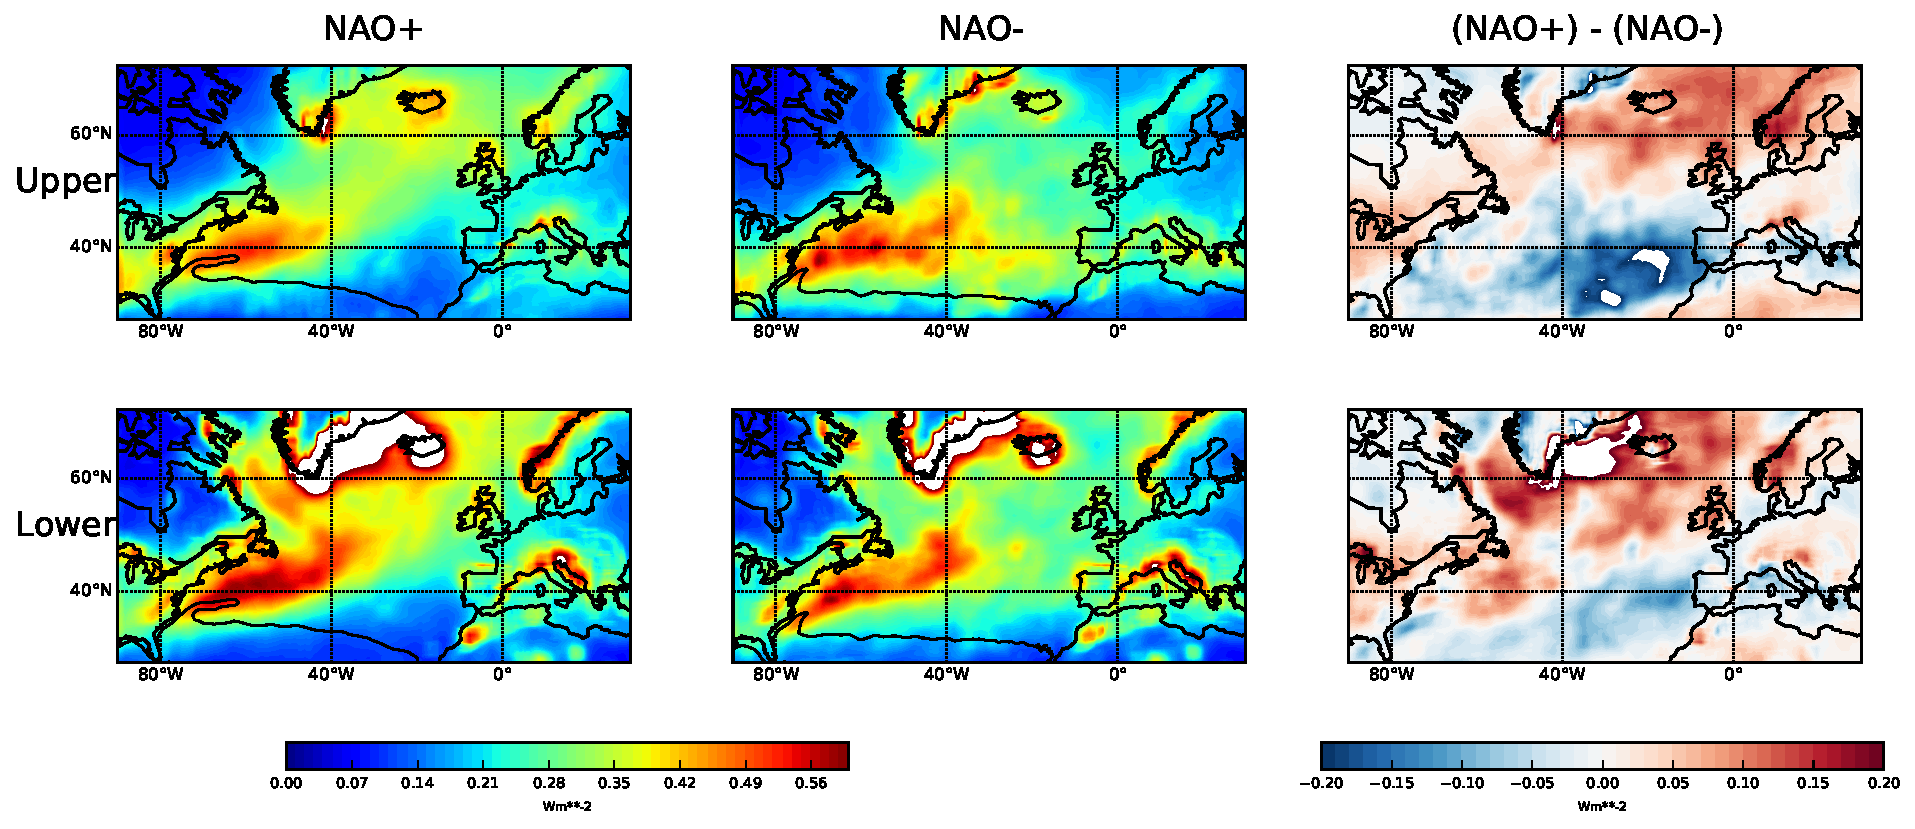
\includegraphics[width=32pc]{ERA5_6buoy_subplot2.pdf}
	\caption{Distribution of positive buoyancy integrated over the upper atmosphere (300-600 hPa) in (a) positive (b) and negative NAO phases and the lower atmosphere (625-925 hPa) in (d) positive (e) and negative NAO phases. Difference in integrated positive shear production NAO positive-NAO negative in the (c) upper atmosphere and (f) lower atmosphere. The 21 $^{0}$C SST isotherm is shown in black contours. At positive saturation, white is shown.}
	\label{fig:ERA5_buoy}
\end{figure}


%%%%%%%%%%% Heat flux %%%%%%%%%%%%%%%%%%%%%%
\begin{figure}[h]
	\centering
	\includegraphics[width=32pc]{ERA5_heatflux_subplot.png}
	\caption{Distribution of surface heat flux a) sensible b) latent in (d) positive (e) and negative NAO phases. Difference in integrated positive shear production NAO positive-NAO negative . The 21 $^{0}$C SST isotherm is shown in black contours. At positive saturation, white is shown. REVERSE 'DIFFERENCE' COLORBAR? BECAUSE MORE HF in -ve, but as it is negative HF, it looks opposite}
	\label{fig:ERA5_hf}
\end{figure}

%%%%%%%%%%%%%%%%%%%%%%%%%%%%%%%%%%%%%%%%%%%%%%%%%%%%%%%%%%%%%%%%%%%%%

%The lower atmosphere more intense than the upper atmosphere.
%In positive NAO years, the UK and Norway experience higher values of positive shear production.
For the shear production term, a zonal extension is observed in NAO-, especially in the upper atmosphere (figure \ref{fig:ERA5_shear}), consistent with the pattern of buoyancy. Shear production is approximately 25\% weaker than buoyancy. Over the warm tongue region, shear production is displaced further northeast in NAO+, along the axes of the extended warm tongue. The largest values of shear production are over high orography, particularly Greenland, where white is color bar saturation. Away from these regions, the most intense values are downstream of the warm tongue, where there is also the maximum difference in the lower atmosphere.


%In the lower atmosphere, that amplitude of the instability is comparable to in the upper atmosphere and the difference between NAO phases shows the same broad pattern, with slightly reduced difference in magnitude. 

\begin{figure}[h]
	\centering
	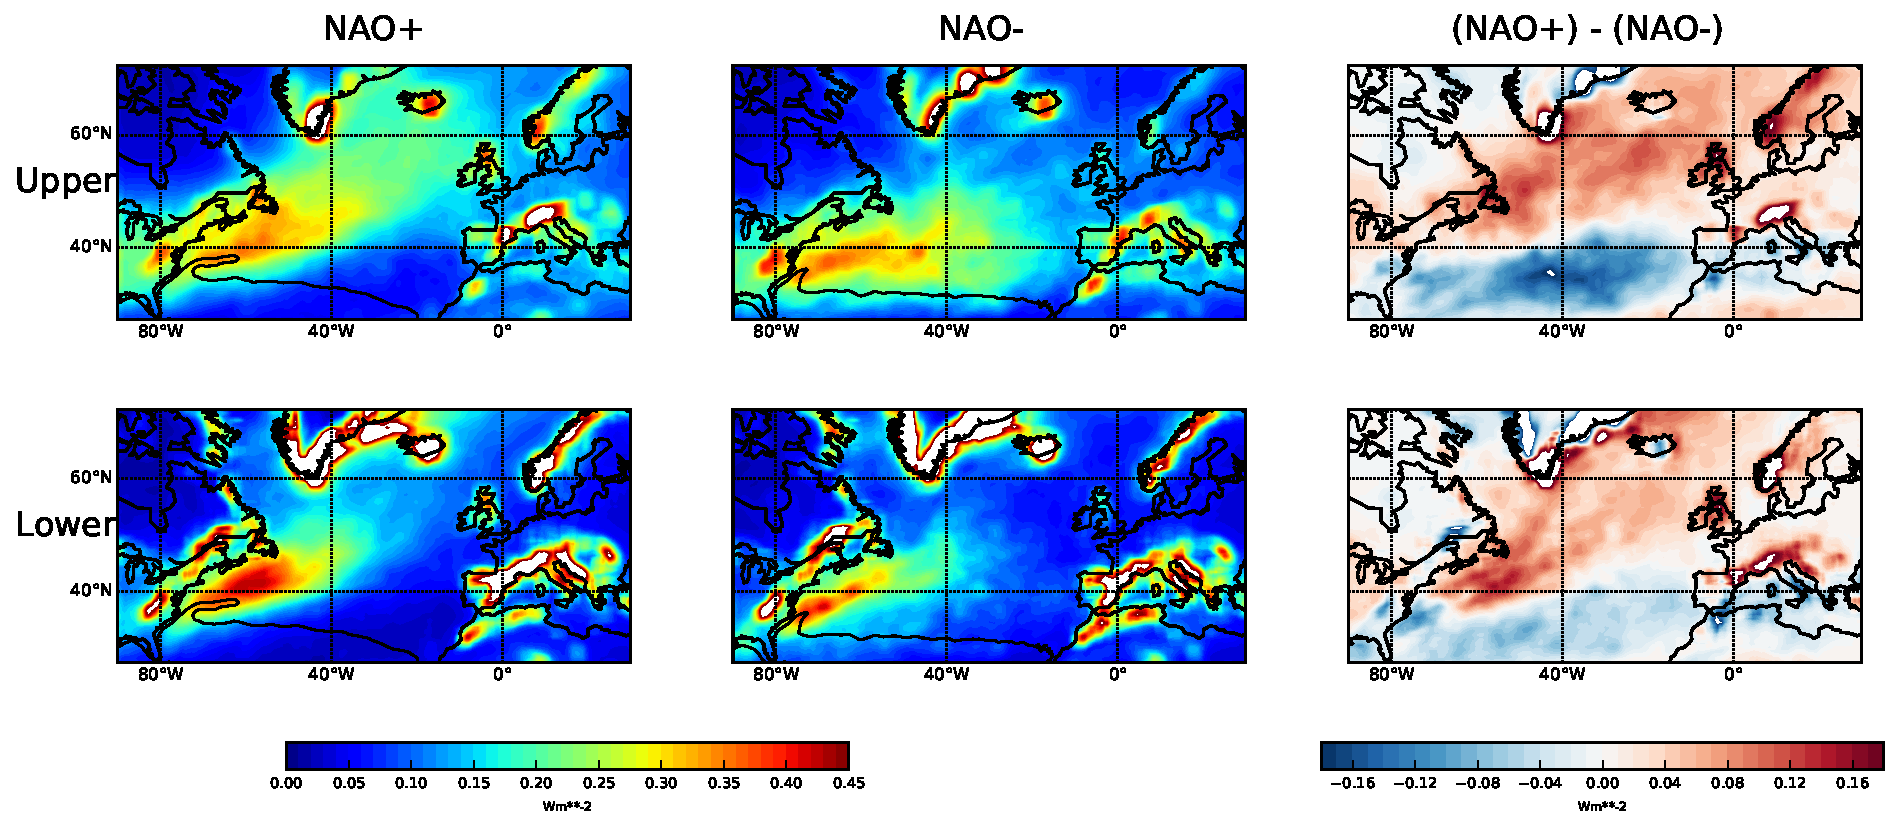
\includegraphics[width=32pc]{ERA5_6shear_subplot2.pdf}
	\caption{Distribution of positive shear production integrated over the upper atmosphere (300-600 hPa) in (a) positive (b) and negative NAO phases and the lower atmosphere (625-925 hPa) in (d) positive (e) and negative NAO phases. Difference in integrated positive shear production NAO positive-NAO negative in the (c) upper atmosphere and (f) lower atmosphere. The 21 $^{0}$C SST isotherm is shown in black contours. At positive saturation, white is shown.}
	\label{fig:ERA5_shear}
\end{figure}

The vertical distribution of buoyancy and shear production is relatively homogeneous throughout the troposphere, with peaks around 500 400 hPa.

The \citet{sheldon2017warm} study found a value of approximately 5 mW/kg at 5 km at one time step. Here, the maximum value over the Gulf Stream region is ~ 40 times weaker. There are model difference, including a doubling of resolution in this study from 12 km in Sheldon to 25$^{0}$ in ERA5. Also this result takes an average over 10 levels, which were interpolated from ..., where any positive value was taken into the mean for each phase. Also this analysis over DJF picks up storms at all stages of their life cycle, perhaps when this instability was weaker than in the single Sheldon experiment. Analysis of the distribution of shear instability values revealed that 5mw/kg could be achieved, but with a probability of ..percent. amplitude of anomaly or difference or total value?
Note that in both my subsets, there is a GS warm tongue (unlike Sheldon experiment, where one is smoothed).
This upper atmosphere slice included 500 hPa, which is comparable to 5 km, where \citet{sheldon2017warm} found the maximum of shear instability in the vertical. 


%%%%%%%%%%%%%%% PV %%%%%%%%%%%%%%%%%%

\begin{figure}[h]
	\centering
	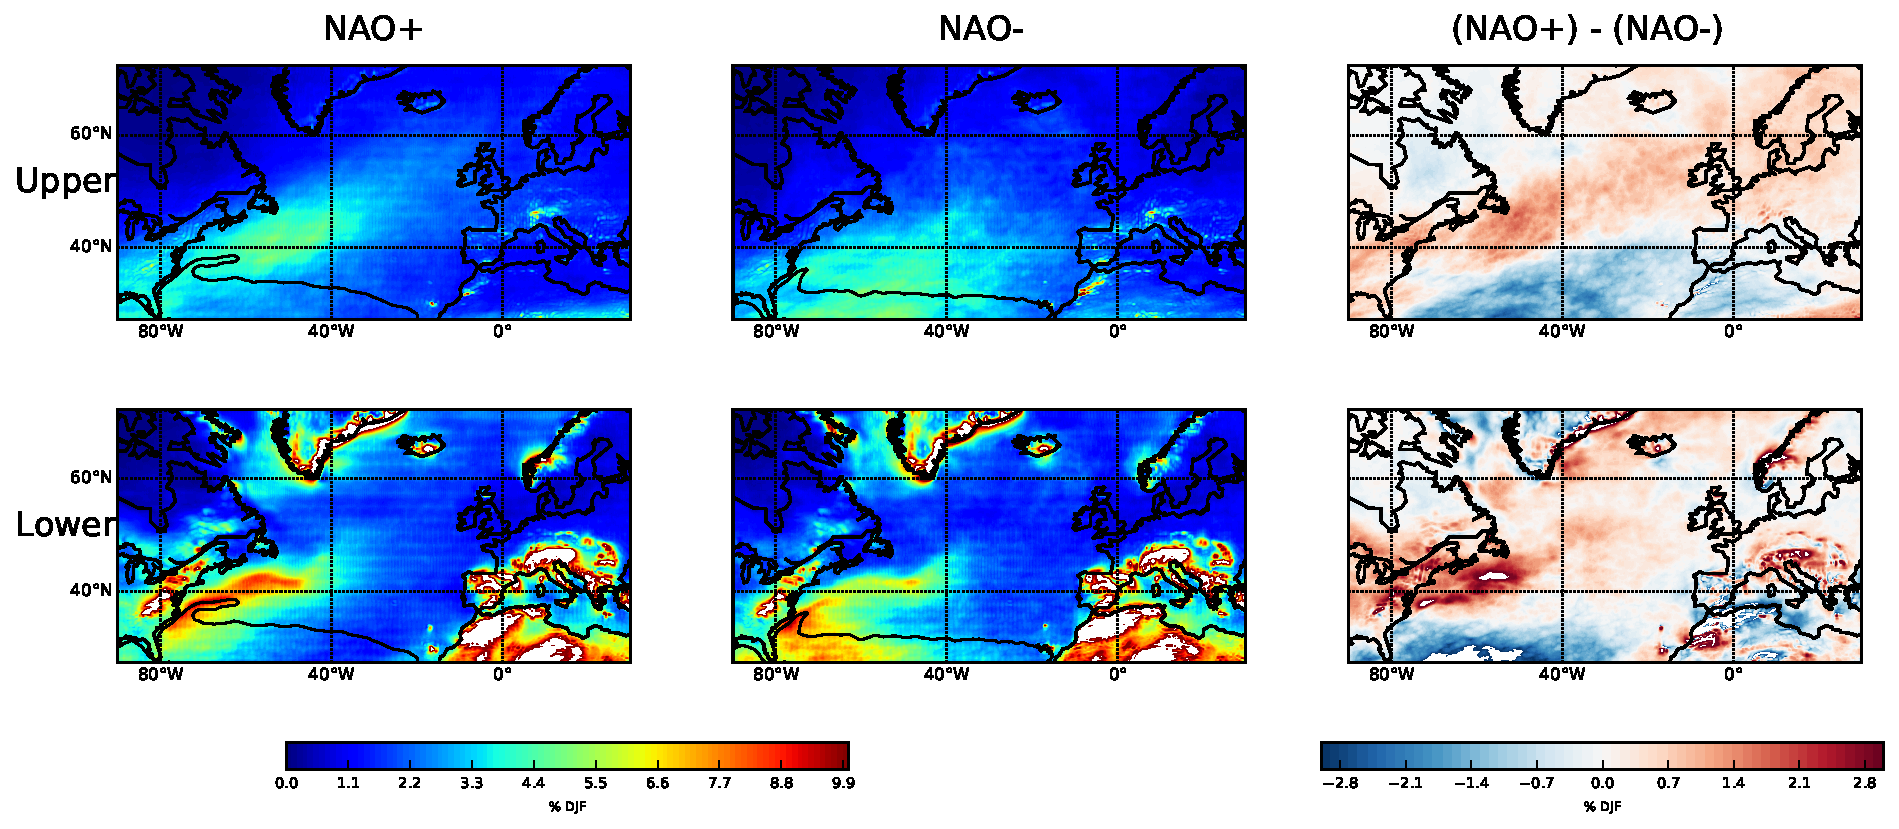
\includegraphics[width=32pc]{ERA5_6PV_subplot2.pdf}
	\caption{Frequency (percentage of DJF) of negative PV averaged over the upper atmosphere (300-600 hPa) in (a) positive (b) and negative NAO phases and averaged over the lower atmosphere (625-925 hPa) in (d) positive (e) and negative NAO phases. Difference in frequency of negative PV NAO positive-NAO negative in the (c) upper atmosphere and (f) lower atmosphere. The 21 $^{0}$C SST isotherm is shown in black contours. At positive saturation, white is shown.}
	\label{fig:ERA5_PV_count_cent}
\end{figure}

\begin{figure}[h]
	\centering
	\includegraphics[width=32pc]{ERA5_PV_300_subplot.png}
	\caption{Mean PV at 300 hPa in (a) positive (b) and negative NAO phases Difference in frequency of negative PV NAO positive-NAO negative in the (c) . The 21 $^{0}$C SST isotherm is shown in black contours. At positive saturation, white is shown. CHECK COLOURS IF WANT TO USE THIS - LOOKS OPPOSITE TO FIG 6}
	\label{fig:ERA5_PV_mean}
\end{figure}

Figure \ref{fig:ERA5_PV_count_cent} shows the frequency (as percentage of DJF) of occurrence of negative potential vorticity (PV) averaged over upper and lower levels. \citet{vanniere2016potential} showed that negative PV generated within the cold sector of extra-tropical storms is present (GS region?) approximately 10-12\% of the time. Averaged over levels in the upper atmosphere negative PV is present 3-4\% of DJF, and in the lower atmosphere is approximately double, frontal occurrence, rapid ascent. We observe the smaller scale signal at low levels, with 'downstream anchoring’ effect of the warm tongue. The presence of negative PV in the upper atmosphere over land is absent, whereas there was strong positive shear production. This suggests that the shear production was mountain wave drag over regions of high orography. Mean negative PV maps have the same spatial distribution as  \ref{fig:ERA5_PV_count_cent}, but larger values in upper levels.

SHOULD I EVEN SHOW THIS AVERAGED LEVEL PV PLOT, OR JUST 950 and 300? STACKED PLOT SHOWS NOTHING GOING ON AT INTERMEDIATE LEVELS, SO MAYBE NOT WORTH SHOWING?

\begin{figure}[h]
	\centering
	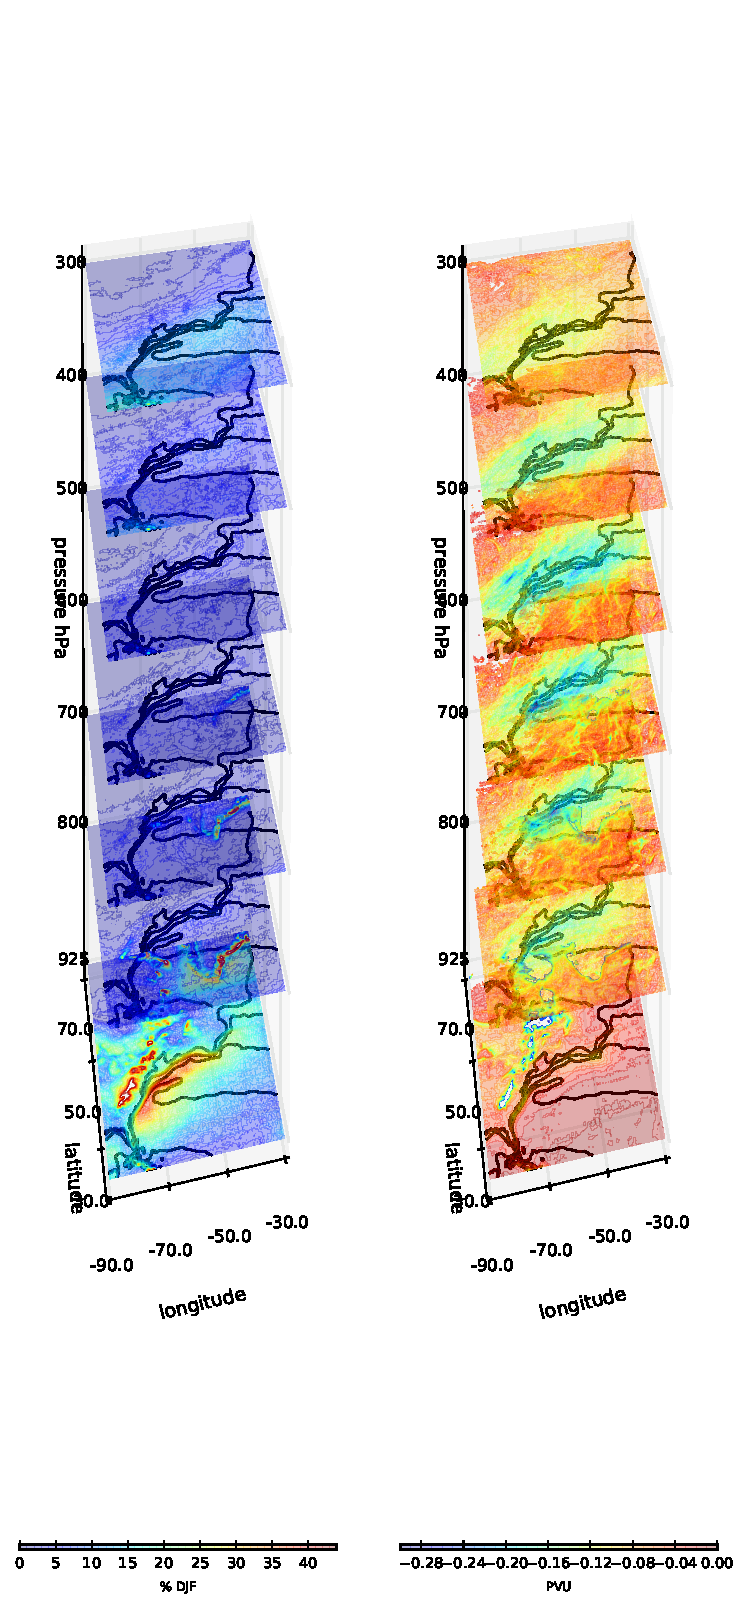
\includegraphics[width=14pc]{ERA5_PV_stack_subplot_NAOpos.pdf}
	\caption{Stacked contour plot of a) negative PV frequency and b) mean negative PV at 925, 800, 700, 600, 500, 400, 300 hPa with SST contour lines.}
	\label{fig:ERA5_PV_stack}
\end{figure}

 \begin{figure}[h]
 	\centering
 	\includegraphics[width=14pc]{ERA5_PVneg_hist_log_NAOpos_300_600_925.pdf}
 	\caption{POSSIBLY COMBINE HISTOGRAM IN SUBPLOT WITH STACKED PLOT. Distribution neg PV NAO pos. 80-40W 30-60N}
 	\label{fig:ERA5_PV_dist_NAOpos}
 \end{figure}

The high frequency of negative PV in the lower levels is dominated by that at 925 hPa (figure \ref{fig:ERA5_PV_stack}, NAO+). The southeastward advection of continental air over the ocean by an extra-tropical cyclone will generate a cold air outbreak, and production of negative PV, but not all storms generate a front large enough to be counted by the frontal detection studies. This stacked plot shows the same vertical structure in the NAO negative years. Throughout the rest of the troposphere, the frequency is consistently lower, but with a relative increase at the 300 hPa. The mean value of negative PV at each layer shows the opposite pattern, with largest magnitude in the mid layers. Strong ascent required to bring the PV all the way to 300hPa are much less frequent than the cold air outbreak. The middle layers hardly keep track of this because of fast ascent, while the spreading at upper levels allow it to be seen there. (Talk about histogram distribution (not shown)?)

%Figure \ref{fig:ERA5_PV_count_cent} shows relatively frequent negative PV at low latitudes and across much of the western part of the Atlantic basin in NAO-. 

The mean total, including positive and negative values at 300 hPa (figure \ref{fig:ERA5_PV_mean}) highlights the strong PV gradient in NAO+ and lower values of PV in the northwest and southeast of the domain in NAO-. The mesoscale activity might strengthen the PV front in NAO+ by injecting low PV at the right place and so feedbacks positively on NAO+; likewise in NAO- it might reinforce the NAO- by injecting low PV in the range of latitude where there is low PV.
Isobaric and isentropic maps looks the same.
Speculation of PV pathway

\begin{figure}[h]
	\centering
	\includegraphics[width=30pc]{Sub_overlay_GS.pdf}
	\caption{a)NAO+ b)NAO-. SST (black), PV (magenta), Shear, Buoyancy. Single contour of each variable. Maybe put in supplementary or delete}
	\label{fig:ERA5_overlay}
\end{figure}

%%%%%%%%%%%%%%%%%%%%%%%%%%%%%

%%%%%%%%%%%%%%%%%%%%%%%%%%%%%%%%%%%%%%%%%%%%%%%%%%%%%%%%%%%%%%%%%%%%%

% \begin{figure}[h]
% 	\centering
% 	\includegraphics[width=20pc]{ERA5_PVneg_hist_log_NAOneg_300_600_925.pdf}
% 	\caption{Distribution neg PV NAO neg}
% 	\label{fig:ERA5_PV_dist_NAOneg}
% \end{figure}

% \begin{figure}[h]
% 	\centering
% 	\includegraphics[width=40pc]{ERA5_6PV_mean_subplot.png}
% 	\caption{CHOOSE EITHER MEAN NEG PV OR NEG PV COUNT. Distribution of mean negative PV in the upper atmosphere (300-600 hPa) in (a) positive (b) and negative NAO phases and in the lower atmosphere (625-925 hPa) in (d) positive (e) and negative NAO phases. Difference in  mean negative PV NAO positive-NAO negative in the (c) upper atmosphere and (f) lower atmosphere. The 21 $^{0}$C SST isotherm is shown in black contours. At positive saturation, white is shown.}
% 	\label{fig:ERA5_PV_mean}
% \end{figure}

% \begin{figure}[h]
% 	\centering
% 	\includegraphics[width=14pc]{ERA5_PV_stack_subplot_NAOneg.pdf}
% 	\caption{SHOW EITHER NAO POS OR NAO NEG OR SUM OF ALL YEARS. Multi layer contour plot of negative PVU count for positive NAO years DJF from hourly ERA5 data.}
% 	\label{fig:ERA5_PVU_NAOneg}
% \end{figure}

% \begin{figure}[h]
% 	\centering
% 	\includegraphics[width=10pc]{GS_stack_ERA5_shear_diag_DJF_pos_mean_NAOneg.pdf}
% 	\caption{Multi layer contour plot of negative shear diag for positive NAO years DJF from hourly ERA5 data.}
% 	\label{fig:ERA5_PVU_shear_diag_layer_NAOpos}
% \end{figure}

%%%%%%%%%%%%%%%%%%%%%%%%%%%%%%%%%%%%%%%%%%%%%%%%%%%%%%%%%%%%%%%%%%%%%

%%%%%%%%%% ERA-Interim %%%%%%%%%%%%%%%%%

The ERA-Interim dataset starts in 1979 and so provides an opportunity to conduct this same analysis over a longer period, with an increased sample size of NAO+ and NAO- years. However, the atmospheric resolution is coarser than ERA5, at 0.75 $^{0}$ rather than 0.25 $^{0}$. Although the atmospheric model resolution is constant throughout the whole data set, the prescribed SST data has changed. ERA-Interim data is analysed from 2002-2018, when the SST resolution is at least as fine as the atmospheric resolution. In years prior to this, the SST is coarse and ....

The same analysis conducted with ERA-Interim 6-hourly data revealed the same spatial pattern in buoyancy and positive shear production with NAO phase, but with differences in magnitude. In ERA-Interim, the values as well as differences of shear and buoyancy production approximately halved. Expected in a coarser resolution model. By definition of these diagnostics (equations \ref{eq_diag2}, \ref{eq_diag3}) and the region size over which the bars and primes are calculated (3 degrees), there will be more production in ERA-5, where 13 grid points have been used, whereas only 5 are used in ERA-Interim.
Three times coarser but only twice as weak?? ERAI uses 6-hourly vs hourly in ERA5!

ERA-Interim, see mesoscale signal when use 20 NAO+ and 8 NAO-.

\begin{figure}[h]
	\centering
	\includegraphics[width=32pc]{ERA_6shear_subplot.pdf}
	\caption{ERA-Interim: Distribution of positive shear production integrated over the upper atmosphere (300-600 hPa) in (a) positive (b) and negative NAO phases and the lower atmosphere (625-925 hPa) in (d) positive (e) and negative NAO phases. Difference in integrated positive shear production NAO positive-NAO negative in the (c) upper atmosphere and (f) lower atmosphere. The 21 $^{0}$C SST isotherm is shown in black contours. At positive saturation, white is shown.}
	\label{fig:ERA_shear}
\end{figure}


Analysis over the full time period includes 20 NAO+ winters and 8 NAO-, four times the number of years in each phase.

  \begin{table}
  \caption{NAO positive and negative winters} \label{t_NAO}
  \centering
  \begin{tabular}{c c c c c c}
  \hline
  \textbf{Positive} & 2011--2012 & 2013--2014 & 2014--2015 & 2015--2016 & 2016--2017 \\
  \hline
  \textbf{Negative}  & 2009--2010  & 2010--2011 &  &  &  \\
  \hline
  \end{tabular}
  \end{table}



ERA5 uses SSTs from HadISST version 2 0.25$^{0}$(Kennedy et al. 2016) to 2007, and thereafter OSTIA 0.05$^{0}$.
%ERA-Interim SST change and effect on air-sea interaction \citet{parfitt2017impact}
%Late 2018	Complete the release of 1979-2009

%%%%%%%%%%%%%%%%%%%%%%%%%%%%%%%%%%%%%%%

\section{Discussion and conclusions}

This observational study uses high resolution data to investigate mesoscale signatures of the North Atlantic Oscillation (NAO) in the atmosphere and ocean.  The distribution of mesoscale buoyancy, shear production and negative potential vorticity (PV) in the atmosphere, along with sea surface temperature (SST) and surface currents in the ocean are described, and a difference with NAO phase is found.
In positive NAO winters, embedded within the large-scale SST tripole is a warming and extension of the Gulf Stream warm tongue, along with a displacement and acceleration of surface currents. Atmospheric mesoscale buoyancy and shear production are anchored downstream of this region, suggesting an 'active' relationship with the underlying ocean, in contrast to the 'passive' mesoscale signal of the large-scale shift of storm track. 
This study highlights the importance of high resolution products to investigate mesoscale phenomena and their (different?) mechanisms.

%relation to NAO phase in the new ERA5 reanalysis, and proposes a positive feedback with the Gulf Stream warm tongue.  It is found that shear instability, like buoyancy, is related to NAO state as it is tightly coupled to the storm track.

%In agreement with a previous experimental study \citet{sheldon2017warm}, this mesoscale SST signature gives rise to an increase in shear instability downstream, with the associated injection of negative potential vorticity air at high levels.

%The positive NAO drives the tripole SST pattern and, we find, also a strengthening of the Gulf Stream warm tongue. Such an SST distribution leads to more shear instability downstream of the warm tongue, opening the possibility of a positive feedback between the ocean on the NAO on scales smaller than those having been discussed so far in the literature.

%This behaviour has been proposed in previous studies, but until now has not been diagnosed in a high resolution reanalysis or with this shear instability.


While previous studies have examined the NAO large-scale tripole in SST, this study has shown a smaller scale feature embedded within. We then show that there is a 'passive' signal in atmospheric buoyancy and shear production aligned with the storm track on the large scale, and also a more localized 'active' relationship with NAO phase over the warm tongue region, motivated by the experiments in \citet{sheldon2017warm}.

*SST pattern: possibly we’re seeing something quite different from previous studies (de Coetlogon and Frankignoul, 2001; Sasaki et al., 2011) because of the persistent NAO+ conditions since ~2010, strongest warm tongue in 1617.

*short dataset

A key issue is whether it matters for the NAO and for seasonal to decadal prediction. Negative PV can be found in the cold sector of extratropical cyclones, and can affect locking frequency and lifetime. If PV<0 is injected at the right place in NAO- to sustain more frequent blocks it may be a mechanism.

%At a localized scale over the Gulf Stream warm tongue, the production terms are displaced in NAO phase in relation to the warm tongue structure \todo{see final new plot}


This hypothesis warrants further investigation through a modeling study at high resolution (at least 0.25$^{0}$) run for climatological time scales to examine the causal relationships between these two variables... Experiment isolate the mechanism.

In summary, this analysis shows the presence of mesoscale signatures in the NAO, with the atmospheric feature anchored downstream of that in the ocean (figures \ref{fig:ERA5_buoy} and \ref{fig:ERA5_shear}). We suggest that this relationship between the atmosphere and  Gulf Stream warm core is 'active', based on results from \citet{sheldon2017warm}, in contrast to the 'passive' mesoscale signal of the large-scale shift of storm track. Highlights the importance of high resolution, able to resolve.../represent... mesoscale... ERA-I and ERA5 have same, high resolution SST, but different atmosphere. Too fine for them, especially ERA-I.

% this observational study using a modern reanalysis suggests the possibility of a positive feedback between the ocean on the NAO on scales smaller than those having been discussed so far in the literature.

%%%%%%%%%%%%%%%%%%%%%%%%%%%%%%%%%%%%%%%%%%%%%%%%%%%%%%%%%%%%

The SST front has a substantial impact on the marine atmospheric boundary layer above - how? wind convergence over sst gradient (Chelton et al., 2004).

Thought confined to boundary layer, but can see throughout troposphere - can we see this in ERA-I?

% Isla Simpson: recent paper:
% "While the above analysis leads us to conclude that the multi-decadal variabilty in March U700 504 is m


 strongly connected with the AMV, some ambiguity remains over the causal nature of this 505 connection. It is well known that variability in the North Atlantic atmospheric circulation and 506 associated surface fluxes is, itself, a driving force for North Atlantic SST variability (Deser and 507 Blackmon 1993; Deser et al. 2010), whether it be through the influence on the deep ocean circula508
% tion (Eden and Jung 2001; Danabasoglu et al. 2014; Yeager and Danabasoglu 2014; Delworth and 509 Zeng 2016; Delworth et al. 2017) or direct influence on the ocean mixed layer (Seager et al. 2000; 510 Clement et al. 2015; Cane et al. 2017). It is, therefore, plausible that these connections indicate 511 a causal link in the opposite sense i.e., the multi-decadal variability in the winds is driving the
% 512 multi-decadal variability in the SSTs. While the coupling between ocean and atmosphere likely 513 goes both ways, we summarize here various lines of reasoning  that support a directed causal link 514 between the SST variability and March U700 in the sense of the SSTs driving March U700.
% The conventional view of North Atlantic ocean-atmosphere coupling, however, is that the pri624
% mary direction of interaction is the opposite of this, with the winds influencing the SSTs. Evidence
% 625 for a connection in the other direction, during winter, is somewhat patchy. It has been argued that North Atlantic SST variability may influence the North Atlantic jet
% 694 through a stratospheric pathway (Omrani et al. 2014).  Indeed,
% 707 recent studies have suggested that improved resolution of ocean fronts and the overlying atmo708
% sphere could significantly alter the nature of ocean-atmosphere coupling (Smirnov et al. 2015;
% 709 Parfitt et al. 2016; Siqueira and Kirtman 2016)."

shear instability = barotropic?

\todo{Things to mention: significance, geostrophy, ocean-atmosphere coupling in the mid-latitudes, mesoscale.}
\todo{Visbeck, Sasaki, Marshall, Cassou, Fan \& Schneider, Small, Bryan, Rodwell, Peng, Wang, Ma, Czaja. Bishop: ocean weather}

%Why does shear production not also happen in this region where there are warmer waters in the positive phase? need some buoyancy to get shear? look at relationship / correlation between buoyancy and shear. too stable over warm waters, do not get shear production either?
% novel approach
%entirely consistent with a feedback
%Negative PV has been reported in the cold sectors of extratropical cyclones (Stoelinga, 1996; Chagnon et al., 2013). Chagnon et al. (2013)showed that negative PV arose from the boundary-layer tendencyand was generated by strong positive heat flux (maximum atthe surface).
%In boreal winter, cold air outbreaks are common in the Western North Atlantic, leading to large heat transfer as this air passes over the warm waters of the Gulf Stream (Zolina and Gulev, 2003).



%Over the North Atlantic, the dominant mode of atmospheric variability is the NAO, which is associated with a latitudinal displacement of the jet. We find that winters associated with a negative phase of the NAO are related to reduced EKE over the Atlantic (not shown), suggesting that a midwinter minimum is more likely to occur in the Atlantic during years of negative NAO. In our analysis, most years of strong jet are associated with negative NAO in winter (five out of seven), and years of weak jet are associated with positive NAO (six out of seven).

%has a (significantly different) spatial distribution in a high resolution reanalysis depending on NAO state. The positive NAO drives the tripole SST pattern and, we find, also a strengthening of the Gulf Stream warm tongue. Such an SST distribution leads to more shear instability downstream of the warm tongue.


########################

\section{Abbreviations}
%http://tex.stackexchange.com/questions/74353/what-commands-are-there-for-horizontal-spacing

% Acronyms



\newpage




\section{Estimate the impact of the new mechanism on the climatological mean state of the North Atlantic}

\subsection{ Hypothesis / Aim}
Develop a simple theoretical model of the findings in Part 1 and 2



%\begin{figure}	
%	\includegraphics[width=34pc,angle=0]{Y:/Code_Data/Plots_new/ECMWF/120104_maps/calcs/masksq_poly_time_diag-precip-msl_ens9_12012004.pdf}
%	\caption{Data}\label{fig:data}
%	\centering
%\end{figure}


%I will assess whether or not the warm path mechanism (Section 3.3), examined in the Met Office case study \cite{sheldon2017warm} and in section \ref{Ch2}, has relevance to the climatological state of the storm-track in the North Atlantic

I will examine the relationship between cyclone activity in the North Atlantic and the sea surface temperature in the Gulf Stream region. I will also estimate the impact of shear instability and slantwise convection on the climatological mean state of the North Atlantic. It is well established that many forecast busts over Europe are due to poor representation of atmospheric blocking \cite{rodwell2013characteristics}. It is also known that blocking and the state of the North Atlantic Oscillation (NAO) are related to storm track activity \citep{vallis2008local}. In this study, I propose that the small-scale mechanism of shear instability is a missing process in climate models, which can have a detrimental effect on the downstream forecast.

%
%Recent numerical experiments with high horizontal resolution (grid spacing of 25km or less) have suggested that the impact of the Gulf Stream on the “storm track” is mediated by the frontal circulation embedded in extra-tropical cyclones. In a series of controlled experiments with the UK Met Office Model, we were able to show that the frontal circulation can be destabilized by the Gulf Stream, with associated injection of low potential vorticity air at upper levels and a potential impact on blocking events further downstream, but we could not assess whether this effect was systematic (Sheldon et al., 2017). In this work, we address this issue by analysing an 11-member ensemble hindcast from ECMWF over the period 2007-2017 at a horizontal resolution of 16km. A large spread is found amongst ensemble members suggesting that, rather than systematically affecting the frontal circulation of cyclones, the effect of the Gulf Stream on them has to be understood within a statistical framework. 

\section{Aims}
\begin{itemize}
	\item Analyse operational forecasts, ensemble hindcasts and reanalysis run at ECMWF (1996 to present) using the shear instability diagnostic
	\item Explore the relationship between shear instability and state of the Gulf Stream
	\item Determine the impact of shear instability in extra-tropical cyclones on the downstream weather over western Europe
	\item Examine the upstream storm track activity (and shear instability) associated with forecast busts in terms of blocking indices
\end{itemize}


%Gerber and Valis 2009

%Unlike upright convection, slantwise convection transports air from low levels at one latitude to high levels at a different latitude. 

% http://www.atmo.arizona.edu/students/courselinks/spring16/atmo541b/handouts/pv_climo_bluestein1992.png

%\begin{figure}[h]
%	\centering
%	\noindent\includegraphics[width=18pc]{H:/Documents/Thesis/phd-thesis-template-2.2.2_AC/phd-thesis-template-2.2.2/Figs/Hoskins_PVview.png}
%	\caption{A schematic view of potential vorticity in the atmosphere. Isentropes every 30 K marked. Tropopause in thick black line. (what PV value?). The arrow indicate some boundaries. The equatorial boundary is defined by the zero PV contour. Source: \cite{hoskins1991towards}} \label{fig:PV_profile}
%\end{figure}

%Time series data downloaded 4th Oct https://www.esrl.noaa.gov/psd/gcos_wgsp/Timeseries/NAO/
%East Atlantic from http://www.cpc.ncep.noaa.gov/data/teledoc/ea.shtml
%Gulf Stream northern wall from PML http://www.pml-gulfstream.org.uk/data.htm

I will analyse hindcasts from 1996-2017 for DJF only. This data will come from hindcasts run on 26 dates (table \ref{t_winterdates}). To focus on the highest resolution sections of these runs (0.2$^0$), I will just retain the first 15 days.

\begin{table}[h]
	\caption{DJF hindcast dates 2016-2017. A total of 26 hindcast dates}\label{t_winterdates}
	\begin{center}
		\begin{tabular}{c}
			%	\begin{tabular}{cc}
			\hline\hline
			Mondays \\
			05/12, 12/12, 19/12, 26/12, 02/01, 09/01, 16/01, 23/01, 30/01, 06/02, 13/02, 20/02, 27/02 \\ 
			\hline
			Thursdays \\			
			01/12, 08/12, 15/12, 22/12, 29/12, 05/01, 12/01, 19/01, 26/01, 02/02, 09/02, 16/02, 23/02  \\ 			
			\hline
		\end{tabular}
	\end{center}
\end{table}

%There are 31 times and 20 years and levels 400, 500, 700. Interpolate to get level 600.
Figure \ref{t_winter_timeline} illustrates the many runs that will be analysed. At times there will be runs initialised on 5 different dates that are representing the same time, which will give 55 ensemble members.

\
As well as the ensemble hindcasts that are at 0.2$^0$ resolution, I will also analyse the operational control forecast, which has a different resolution depending on the year (see table \ref{t_ecmwf2}) along with the ERA-Interim renanalysis.
Using such a rich sample allows for both the climatology over a long time period to be examined, and also 
the ensemble spread on shorter timescales.


\section{Method}
Work has begun on downloading the large datasets required. I have also developed a working code for diagnosing atmospheric blocking based on the below.


\subsection{Atmospheric blocking indices}

A blocking time series has been calculated based on the method by \cite{davini2016northern}. To examine blocking over the Euro-Atlantic region, 60W-22.5W is the West Atlantic and 22.5W-45E is the East Atlantic.

$\phi_{0}$ = 60N; $\phi_{S}$ = 41.25N; $\phi_{N}$ = 78.75N; $\Delta$ = -3.75, 0, 3.75

\begin{equation} \label{eqblock1} %%% did not like blank line below - displaymath needs $$
GHGS(\lambda_{0}, \Delta) = \frac{Z500(\lambda_{0}, \phi_{0}+ \Delta) - Z500(\lambda_{0}, \phi_{S}+ \Delta)}
{\phi_{0} - \phi_{S}}
\end{equation}

\begin{equation} \label{eqblock2}
GHGN(\lambda_{0}, \Delta) = \frac{Z500(\lambda_{0}, \phi_{N}+ \Delta) - Z500(\lambda_{0}, \phi_{0}+ \Delta)}
{\phi_{N} - \phi_{0}}
\end{equation}


\begin{equation} \label{eqblock3}
IB(\lambda_{0}) = 1,   \textbf{if for any} \Delta ,  GHGS(\lambda_{0}, \Delta) > 0  , \textbf{and},   GHGN(\lambda_{0}, \Delta) < -5 m 
\end{equation}


This method, like many similar calculate the gradient in geopotential height (z) in a southern and northern region. If the gradient in the southern part is positive (i.e. increased westerlies) and in the northern part is negative (decreased westerlies), then blocking is diagnosed.
%Why 500 hPa?

% http://www.metoffice.gov.uk/learning/learn-about-the-weather/how-weather-works/factors-that-influence-uk-winters

%\begin{figure}[h]
%	\centering
%	\noindent\includegraphics[width=38pc]{H:/Documents/Thesis/phd-thesis-template-2.2.2_AC/phd-thesis-template-2.2.2/Figs/nao_mo.jpg}
%	\caption{NAO}\label{fig:NAO}
%\end{figure}

A sector is considered blocked if at least 11.25 degrees in longitude is consistently blocked. A blocking event requires persistence in time of at least five consecutive days. Figure \ref{fig:block_criteria} shows the GHGS values for 2015. The red box in the bottom left hand corner illustrates the dimensions in time and space that must be satisfied in order for a blocking event to be categorised.
%NB Update plot to plot Hov of combined GHGS A and GHGNA???

%\begin{figure}	
%	\includegraphics[width=22pc,angle=0]{Y:/Code_Data/Chapter2_3/Plots/final/Hovm_GHGNA_2015_area.png}	
%	\caption{Blocking event criteria in space and time}\label{fig:block_criteria}
%	\centering
%\end{figure}

%This blocking index has been calculated using... forecast ? hindcast?

%\begin{figure}
%		\includegraphics[width=22pc,angle=0]{H:/Documents/Thesis/phd-thesis-template-2.2.2_AC/phd-thesis-template-2.2.2/Figs/ens_spread.png}
%	\caption{Blocking events from ...}\label{fig:block_events}
%	\centering
%\end{figure}

%The period being examined initially is 2008-2017 DJF. 



\section{Possible future analysis across thesis chapters 2 and 3}

% https://software.ecmwf.int/wiki/display/CKB/What+is+ERA5

In Q2 2018 a new reanalysis produced by ECMWF will be released. ERA5 is the 5th major global reanalysis produced by ECMWF. Unlike ERA-Interim, which is deterministic, this reanalysis has 10 ensemble members, and also ensemble mean and spread for all parameters and levels are being produced. The horizontal resolution is considerably higher spatial and temporal resolution than its predecessor ERA-Interim: hourly analysis fields are available at a horizontal resolution of 31 km, and on 137 levels from the surface up to 0.01 hPa (around 80 km). In addition, information on uncertainties is provided for each parameter at 3-hourly intervals and at a horizontal resolution of 62 km.
Adding this reanalysis to the suite of data products analysed over a number of years alongside research for Chapter 3, as well as for the single storm analysis for Chapter 2 would be beneficial.
%79 km globally, 60 levels to 0.1 hPa31 km globally, 137 levels to 0.01 hPa
%10-member Ensemble of Data Assimilations (EDA) at 63 km resolutio





%%%%%%%%%%%%%%%%%%%%%%%%%%%%%%%%%%%%%%%%%%%%%%%%%%%%%%%%%%%%%%%%%%%%%
% APPENDIXES
%%%%%%%%%%%%%%%%%%%%%%%%%%%%%%%%%%%%%%%%%%%%%%%%%%%%%%%%%%%%%%%%%%%%%
%
% Use \appendix if there is only one appendix.
%\appendix

% Use \appendix[A], \appendix}[B], if you have multiple appendixes.
%\appendix[A]

%% Appendix title is necessary! For appendix title:
%\appendixtitle{}

%%% Appendix section numbering (note, skip \section and begin with \subsection)
% \subsection{First primary heading}

% \subsubsection{First secondary heading}

% \paragraph{First tertiary heading}

%% Important!
%\appendcaption{<appendix letter and number>}{<caption>} 
%must be used for figures and tables in appendixes, e.g.,
%
%\newpage
%\appendix
%\chapter{Appendix}
%%
%\section{Glossary}
%
%\subsection {Entropy (potential temperature)}
%Potential temperature is a more useful quantity than temperature as it is not affected my vertical movements - expansion and compression of air mass. Also most unstable path? requires no buoyancy. Calculated from temperature and pressure
%
%% used to use the brackets and backslash. Now use equation environment \[\theta =  T \big(\frac{P_0}{P}) ^{0.286} \]
%\begin{equation} \label{eq_theta}
%\theta =  T \big(\frac{P_0}{P}) ^{0.286}
%\end{equation}
%
%\subsection{Equivalent potential temperature:}  commonly referred to as theta-e ($\theta _{e}$), is a quantity that is conserved during changes to an air parcel's pressure (that is, during vertical motions in the atmosphere), even if water vapor condenses during that pressure change. It is therefore more conserved than the ordinary potential temperature, which remains constant only for unsaturated vertical motions (pressure changes). \\
%
%the temperature a parcel of air would reach if all the water vapor in the parcel were to condense, releasing its latent heat, and the parcel was brought adiabatically to a standard reference pressure, usually 1000 hPa (1000 mbar) which is roughly equal to atmospheric pressure at sea level. A thermodynamic quantity, with its natural logarithm proportional to the entropy of moist air, that is conserved in a reversible moist adiabatic process.
%
%
%\subsection{Potential vorticity:} the absolute circulation of an air parcel that is enclosed between two isentropic surfaces. If PV is displayed on a surface of constant potential temperature, then it is officially called IPV (isentropic potential vorticity). the product of absolute vorticity on an isentropic surface and static stability. So PV consists, in contrast to vorticity on isobaric surfaces, of two factors, a dynamical element and a thermodynamical element.
%
%\begin{equation} \label{eq_PV}
%
%PV = -g (\zeta + f)  \frac{\delta \Theta}{ \delta p} 
%
%\end{equation}
%
%The potential vorticity (PV) is the absolute circulation of an air parcel that is enclosed between two isentropic surfaces. If PV is displayed on a surface of constant potential temperature, then it is officially called IPV (isentropic potential vorticity). Of course, PV could also be displayed on another surface, for example a pressure surface. Note from the relation below, that PV is simply the product of absolute vorticity on an isentropic surface and static stability. So PV consists, in contrast to vorticity on isobaric surfaces, of two factors, a dynamical element and a thermodynamical element.

%
%\subsection{Hydrostatic:}
%The atmosphere is in hydrostatic balance when the upward pressure gradient force is balanced by the downward-directed gravitational pull of the Earth, or weight of the air column. On average the Earth’s atmosphere is  close to hydrostatic equilibrium, however, at high resolution (scales of 10 km or less), non-hydrostatic effects become relevant (ref ecmwf web and info from hydro vs non hydro).
%Two-time-level:
%
%Semi-implicit:
%
%Semi-Lagrangian: text book
%Correlation
%Correlation
%Covariance \\




%%%%%%%%%%%%%%%%%%%%%%%%%%%%%%%%%%%%%%%%%%%%%%%%%%%%%%%%%%%%%%%%

%\begin{acronymns}
%	
%	\acro{PV}{text}
%	
%\end{acronyms}
%
%\begin{tabular}{ l l }
%	AGCM & Atmospheric Global Climate Model \\
%	%	D26 & Depth of 26C isotherm \\
%	DLM & Deep layer mean \\ 
%	
%\end{tabular}


\acknowledgments
ECMWF
NAO Index Data provided by the Climate Analysis Section, NCAR, Boulder, USA, Hurrell (2003). Updated regularly. Accessed 17 April 2018.
Magdalena, Frederic, Paul Dando

'Generated using Copernicus Climate Change Service Information [2018]'.
% https://software.ecmwf.int/wiki/display/CKB/ERA5+data+documentation#ERA5datadocumentation-HowtociteERA5

OSCAR citation ESR. 2009. OSCAR third degree resolution ocean surface currents. Ver. 1. PO.DAAC,	CA,	USA. Dataset accessed [YYYY-MM-DD] at http://dx.doi.org/10.5067/OSCAR-03D01.
